% L13a jump hidden Markov model, how the model is fit (November 12, 2026, at the instructor's
% request: "we took a ticker, fit its growth rate series to a cumulative distribution, then
% sliced up the distribution into states, and counted how many times we moved from state to
% state"). Each slice is labeled with a mood, at his request ("each sub-division is a mood").
% Redrawn on November 13, 2026, as variant D of four mock-ups, which he chose: one row, each
% marker shows the state of its day, the moves are drawn on the plot, and the slices are
% equal areas under the fitted Laplace density.
% Redrawn again the same day as variant G, which he chose over D, E, and F:
%  - a wider growth-rate range (F = 0.05 to 0.95), so the tail slices are mostly drawn and
%    look like 20%, and the jump days sit farther out (E);
%  - no count bracket across the top: an orange key in the plot and a short orange count
%    arrow from the state bar to the table (F);
%  - headers that match the step labels of the fitting algorithm: 1. Laplace, 2. States,
%    3. Count, and 4. Transitions on the estimate box.
%
% Left: the daily growth rates of a ticker, with the five state bands shaded behind them.
% Each marker shows the state of its day, and the three moves 3 -> 4 are the orange segments
% of the line. Middle: the fitted Laplace density, drawn sideways on the same growth-rate
% axis and cut into N = 5 slices of equal area (20% each). The bar names the state and the
% mood of each slice. Right: the table of counted moves and the estimate of P.
%
% Consistency checks (by hand):
%  - Laplace scale b = 1.8 about the median at y = 1.8 ln 10 = 4.1447. The boundaries
%    F^{-1}(k/5) sit at the median -/+ 1.8 ln 2.5 = 1.6493 and -/+ 1.8 ln 1.25 = 0.4017:
%    2.4953, 3.7430, 4.5463, and 5.7940. These quantiles make the five slices equal in area.
%    The plot ends at y = 0 and y = 8.2893 (the median -/+ 1.8 ln 10), where F = 0.05 and
%    0.95, so the drawn part of each tail slice holds 15% of its 20%.
%  - Every marker lies in the band of the state written in it (checked by script).
%  - The 15 moves in the sequence 3 4 3 2 3 4 5 1 5 1 2 3 4 3 3 2 give the counts in the
%    table: 1->2 (1), 1->5 (1), 2->3 (2), 3->2 (2), 3->3 (1), 3->4 (3), 4->3 (2), 4->5 (1),
%    5->1 (2). The three 3->4 moves are the orange segments (days 1-2, 5-6, 12-13), and
%    row 3 sums to 6.
%
% Geometry: the plot and the density are drawn in data units under yscale = 0.91, so the
% plot is 7.54 cm tall, as in D. The table and the estimate are drawn in plain centimeters.
% Days sit 0.53 cm apart and the markers are 3.0 mm wide.
\documentclass[tikz,border=6pt]{standalone}
% Shared style for the L13a schematics (November 12, 2026), \input by each Fig-L13a-*.tex.
% Same fonts, ink, accent colors, boxes, and arrows as the L12a schematics
% (week-12/L12a/figs/abm-diagram.tex), with the plot styles of the L10b profit diagrams
% (arrowed axes, a thick ink curve, open circle markers, dashed drops). The notebook SVG
% carries a dark palette added by theme_svg.py; every color here must be mapped there.
\usepackage[no-math]{fontspec}
\IfFontExistsTF{Arial}{\setsansfont{Arial}}{\setsansfont{TeX Gyre Heros}}
\renewcommand{\familydefault}{\sfdefault}
\usepackage{amsmath,amssymb}
\usetikzlibrary{arrows.meta,calc,positioning,decorations.pathreplacing}

\definecolor{vnink}{HTML}{202124}
\definecolor{gdblue}{HTML}{0091FF}
\definecolor{gdred}{HTML}{E02020}
\definecolor{gdgray}{HTML}{6D7278}
\definecolor{saorange}{HTML}{F08C00}
\definecolor{boxfill}{HTML}{F1F3F4}
\definecolor{orangefill}{HTML}{FFE8C7}
\definecolor{bluefill}{HTML}{E5F3FF}
\definecolor{redfill}{HTML}{FDE8E8}
\definecolor{gridgray}{HTML}{E3E5E8}

\tikzset{
  every picture/.append style={x=1cm, y=1cm, font=\sffamily\small, text=vnink},
  % boxes and arrows, as in the L12a schematics
  flow/.style={draw=vnink, line width=0.9pt, -{Latex[length=2.4mm, width=1.7mm]}},
  feedback/.style={draw=saorange, line width=1.2pt, -{Latex[length=2.6mm, width=1.9mm]}, rounded corners=6pt},
  sumbox/.style={draw=vnink, fill=boxfill, line width=0.8pt, rounded corners=3pt, inner sep=5pt, align=center},
  note/.style={text=gdgray, font=\sffamily\footnotesize, align=center},
  state/.style={circle, draw=vnink, fill=white, line width=1.0pt, minimum size=1.1cm, inner sep=0pt, font=\sffamily\normalsize},
  % plots, as in the L10b profit diagrams
  axis/.style={draw=vnink, line width=0.8pt, -{Latex[length=2.6mm, width=1.8mm]}},
  spine/.style={draw=vnink, line width=0.8pt},
  curve/.style={draw=vnink, line width=1.6pt, line join=round, line cap=round},
  series/.style={draw=gdgray, line width=0.9pt, line join=round},
  drop/.style={draw=gdgray, line width=0.8pt, dash pattern=on 3pt off 2pt},
  pt/.style={circle, draw=vnink, fill=white, line width=1.0pt, inner sep=0pt, minimum size=2.0mm},
}


\tikzset{
  daypt/.style={circle, draw=#1, text=#1, fill=white, line width=0.9pt, inner sep=0pt,
    minimum size=3.0mm, font=\sffamily\scriptsize},
  move/.style={draw=saorange, line width=2.0pt, line cap=round},
  boundary/.style={draw=gdgray, line width=0.5pt},
}

\begin{document}
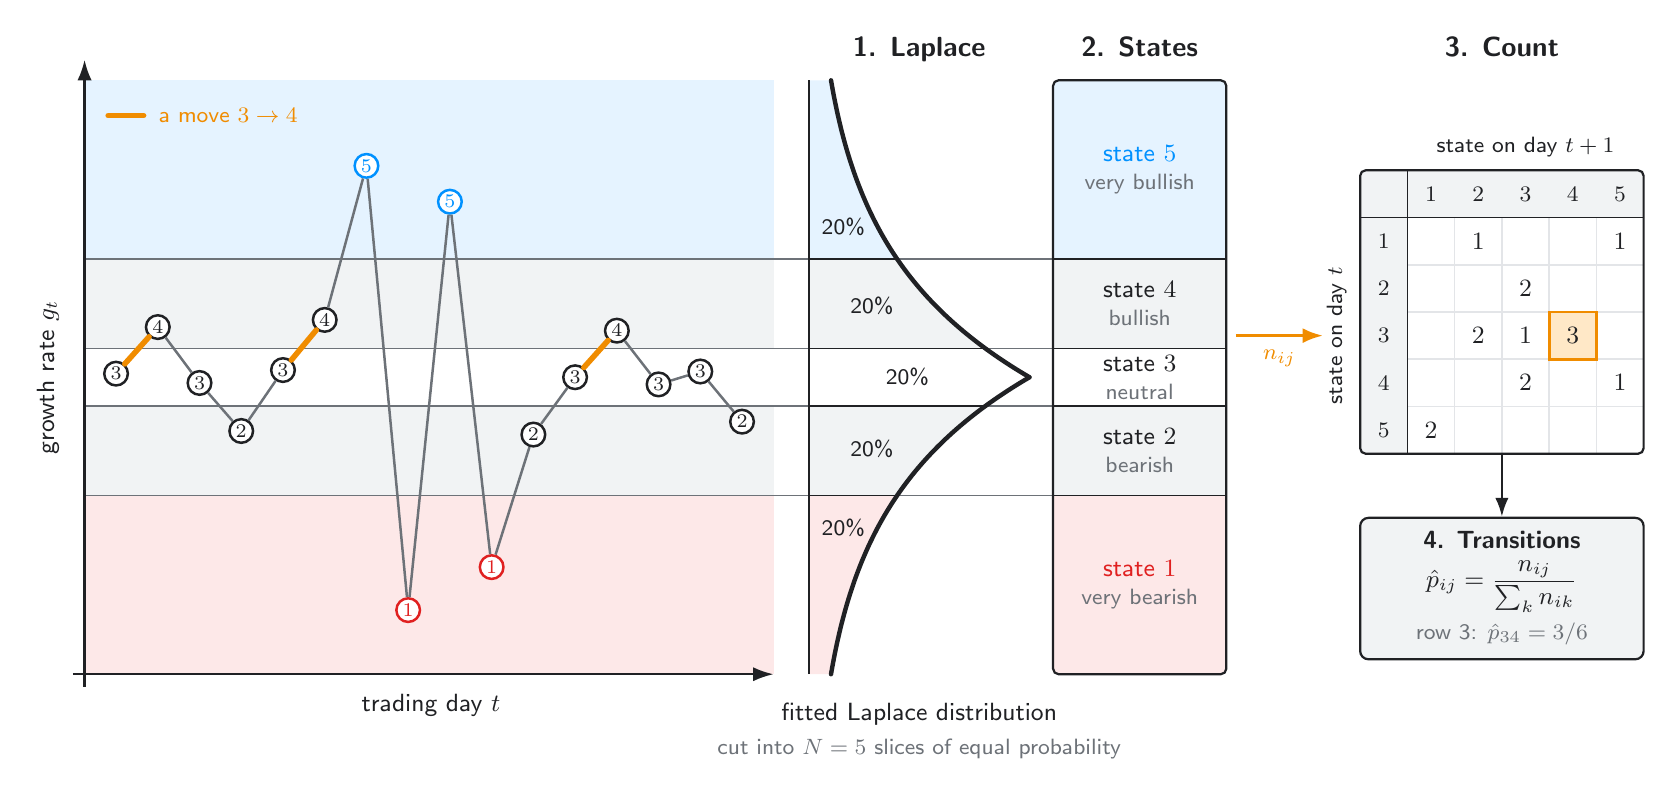
\begin{tikzpicture}

  \begin{scope}[yscale=0.91]

    % ================= the five state bands, across the plot and the distribution =================
    \fill[redfill]  (0, 0)      rectangle (8.75, 2.4953);
    \fill[boxfill]  (0, 2.4953) rectangle (8.75, 3.743);
    \fill[boxfill]  (0, 4.5463) rectangle (8.75, 5.794);
    \fill[bluefill] (0, 5.794)  rectangle (8.75, 8.2893);
    \foreach \y in {2.4953, 3.743, 4.5463, 5.794} {\draw[boundary] (0, \y) -- (12.3, \y);}

    % ================= left: the growth rates of a ticker =================
    \draw[axis] (-0.15, 0) -- (8.75, 0);
    \draw[axis] (0, -0.1714) -- (0, 8.575);
    \node[anchor=north] at (4.4, -0.1429) {trading day $t$};
    \node[rotate=90, anchor=south] at (-0.2, 4.1447) {growth rate $g_{t}$};

    \foreach \i/\x/\y/\s/\c in {
        1/0.40/4.1947/3/vnink,  2/0.93/4.8447/4/vnink,  3/1.46/4.0647/3/vnink,  4/1.99/3.3947/2/vnink,
        5/2.52/4.2447/3/vnink,  6/3.05/4.9447/4/vnink,  7/3.58/7.0947/5/gdblue, 8/4.11/0.8947/1/gdred,
        9/4.64/6.5947/5/gdblue, 10/5.17/1.4947/1/gdred, 11/5.70/3.3447/2/vnink, 12/6.23/4.1447/3/vnink,
        13/6.76/4.7947/4/vnink, 14/7.29/4.0447/3/vnink, 15/7.82/4.2247/3/vnink, 16/8.35/3.5247/2/vnink} {
      \node[daypt=\c] (d\i) at (\x, \y) {$\s$};
    }
    % the series line, with the three moves 3 -> 4 in orange
    \foreach \a/\b in {2/3, 3/4, 4/5, 6/7, 7/8, 8/9, 9/10, 10/11, 11/12, 13/14, 14/15, 15/16} {
      \draw[series] (d\a) -- (d\b);
    }
    \foreach \a/\b in {1/2, 5/6, 12/13} {\draw[move] (d\a) -- (d\b);}

    % ================= middle: the fitted Laplace density, sideways, cut into equal areas =================
    % spine at x0 = 9.2, peak width A = 2.8 cm: x = x0 + A exp(-|y - 4.1447|/1.8)
    \foreach \ya/\yb/\f in {0/2.4953/redfill, 2.4953/3.743/boxfill, 4.5463/5.794/boxfill,
        5.794/8.2893/bluefill, 3.743/4.5463/white} {
      \fill[\f] (9.2, \ya) --
        plot[domain=\ya:\yb, samples=40, variable=\y] ({9.2 + 2.8*exp(-abs(\y-4.1447)/1.8)}, \y) --
        (9.2, \yb) -- cycle;
    }
    \foreach \y/\w in {2.4953/10.32, 3.743/11.44, 4.5463/11.44, 5.794/10.32} {
      \draw[draw=vnink, line width=0.6pt] (9.2, \y) -- (\w, \y);
    }
    \draw[spine] (9.2, 0) -- (9.2, 8.2893);
    \draw[curve]
      plot[domain=0:4.1447, samples=60, smooth, variable=\y] ({9.2 + 2.8*exp(-abs(\y-4.1447)/1.8)}, \y);
    \draw[curve]
      plot[domain=4.1447:8.2893, samples=60, smooth, variable=\y] ({9.2 + 2.8*exp(-abs(\y-4.1447)/1.8)}, \y);
    % equal areas: each slice holds 20% of the probability
    \foreach \x/\y in {9.636/2.0447, 10/3.1447, 10.45/4.1447, 10/5.1447, 9.636/6.2447} {
      \node[font=\sffamily\footnotesize, inner sep=0pt] at (\x, \y) {20\%};
    }

    % ================= each slice is a state and a mood =================
    \begin{scope}
      \clip[rounded corners=2pt] (12.3, 0) rectangle (14.5, 8.2893);
      \fill[redfill]  (12.3, 0)      rectangle (14.5, 2.4953);
      \fill[boxfill]  (12.3, 2.4953) rectangle (14.5, 3.743);
      \fill[white]    (12.3, 3.743)  rectangle (14.5, 4.5463);
      \fill[boxfill]  (12.3, 4.5463) rectangle (14.5, 5.794);
      \fill[bluefill] (12.3, 5.794)  rectangle (14.5, 8.2893);
    \end{scope}
    \foreach \y in {2.4953, 3.743, 4.5463, 5.794} {\draw[draw=vnink, line width=0.6pt] (12.3, \y) -- (14.5, \y);}
    \draw[draw=vnink, line width=0.8pt, rounded corners=2pt] (12.3, 0) rectangle (14.5, 8.2893);
    \foreach \y/\s/\c/\m in {
        1.2477/1/gdred/very bearish, 3.1192/2/vnink/bearish, 4.1447/3/vnink/neutral,
        5.1701/4/vnink/bullish, 7.0416/5/gdblue/very bullish} {
      \node[align=center] at (13.4, \y) {\textcolor{\c}{state $\s$}\\[-1pt]{\footnotesize\color{gdgray}\m}};
    }

    % the key for the orange moves
    \draw[move] (0.3, 7.7948) -- (0.75, 7.7948);
    \node[anchor=west, text=saorange, font=\sffamily\footnotesize] at (0.82, 7.7948) {a move $3\rightarrow4$};
  \end{scope}

  % ================= the count arrow (plain centimeters from here on) =================
  \draw[feedback] (14.62, 4.3) -- (15.73, 4.3);
  \node[anchor=north, text=saorange, font=\sffamily\footnotesize] at (15.175, 4.24) {$n_{ij}$};

  % ================= right: the counted moves =================
  % columns: header at x = 16.5, then states 1..5 at 17.1, 17.7, 18.3, 18.9, 19.5
  % rows:    header at y = 6.1,  then states 1..5 at 5.5, 4.9, 4.3, 3.7, 3.1
  \begin{scope}
    \clip[rounded corners=2pt] (16.2, 2.8) rectangle (19.8, 6.4);
    \fill[boxfill] (16.2, 5.8) rectangle (19.8, 6.4);
    \fill[boxfill] (16.2, 2.8) rectangle (16.8, 6.4);
  \end{scope}
  \foreach \k in {1,...,4} {
    \draw[draw=gridgray, line width=0.6pt] (16.8, {5.8 - 0.6*\k}) -- (19.8, {5.8 - 0.6*\k});
    \draw[draw=gridgray, line width=0.6pt] ({16.8 + 0.6*\k}, 2.8) -- ({16.8 + 0.6*\k}, 5.8);
  }
  \draw[draw=vnink, line width=0.6pt] (16.2, 5.8) -- (19.8, 5.8) (16.8, 2.8) -- (16.8, 6.4);
  \draw[draw=vnink, line width=0.8pt, rounded corners=2pt] (16.2, 2.8) rectangle (19.8, 6.4);
  \foreach \k in {1,...,5} {
    \node[font=\sffamily\footnotesize] at ({16.5 + 0.6*\k}, 6.1) {$\k$};
    \node[font=\sffamily\footnotesize] at (16.5, {6.1 - 0.6*\k}) {$\k$};
  }
  \draw[draw=saorange, fill=orangefill, line width=1.0pt] (18.6, 4.0) rectangle (19.2, 4.6);
  \foreach \r/\c/\n in {1/2/1, 1/5/1, 2/3/2, 3/2/2, 3/3/1, 3/4/3, 4/3/2, 4/5/1, 5/1/2} {
    \node at ({16.5 + 0.6*\c}, {6.1 - 0.6*\r}) {$\n$};
  }
  \node[anchor=south, font=\sffamily\footnotesize] at (18.3, 6.45) {state on day $t+1$};
  \node[rotate=90, anchor=south, font=\sffamily\footnotesize] at (16.15, 4.3) {state on day $t$};

  % the estimate of the transition matrix
  \node[sumbox, minimum width=3.6cm, anchor=north] (phat) at (18.0, 2.0)
    {{\bfseries 4. Transitions}\\[3pt]$\hat{p}_{ij}=\dfrac{n_{ij}}{\sum_{k}n_{ik}}$\\[3pt]{\footnotesize\color{gdgray}row 3: $\hat{p}_{34}=3/6$}};
  \draw[flow] (18.0, 2.8) -- (phat.north);

  % ================= the step labels of the fitting algorithm =================
  \node[anchor=base, font=\sffamily\bfseries] at (10.6, 7.85) {1. Laplace};
  \node[anchor=base, font=\sffamily\bfseries] at (13.4, 7.85) {2. States};
  \node[anchor=base, font=\sffamily\bfseries] at (18.0, 7.85) {3. Count};

  % the name of the distribution, below it
  \node[anchor=north] at (10.6, -0.25) {fitted Laplace distribution};
  \node[note, anchor=north] at (10.6, -0.7) {cut into $N=5$ slices of equal probability};

\end{tikzpicture}
\end{document}
